\subsection{Risk analysis}
\label{risk}


Table \ref{riskshort} shows the worst risks that we think can go wrong in the project (a full list of risks can be seen in appendix \ref{riskapp}). We have evaluated what consequence these different risks have to the project and the probability for them to happen. To see an illustrative overview of all risks with their respective consequence and probability see figure \ref{cxp}. As seen in the figure we only mention the risks which is in the red area of the diagram.

%\begin{itemize}
%\item[-] 
%\item[-] 
%\item[-] 
%\item[-] 
%\item[-] 
%\end{itemize}

\begin{figure}[h!]
\centering
\label{cxp}
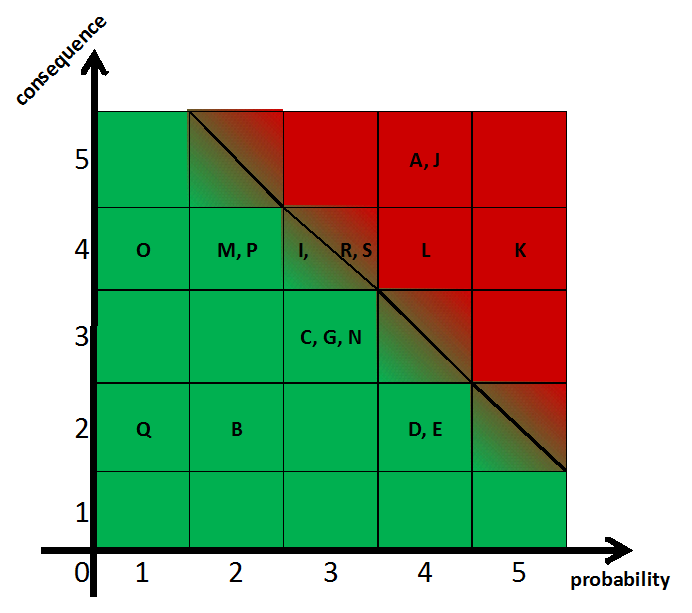
\includegraphics[scale=0.4]{./graphics/cxp}
\caption{Consequence \& probability diagram with placed risks}
\end{figure}

\def\arraystretch{1.7}
\begin{table}[h!]
\label{riskshort}
\centering
\scriptsize
\begin{tabular}{|p{3cm} |p{0.3cm} |p{0.9cm} |p{0.9cm} |p{0.5cm} |p{3cm} |p{3cm} |p{0.7cm}|}
\hline
Risk 	&	No.	& Conse- \newline quence	& Prob-\newline  ability	& CxP	& Initiatives \newline for consequence	& Initiatives \newline for probability	& Cost \newline (DKK) \\
\hline
Cannot access to a credit from investor / bank					& A	& 5				&	4			& 20	& Present the project to more investors or banks	& Develop a good business plan, try to be financed by a company, sell part of the company's benefit	& 0\\
\hline
Subcontractor let down & & & & & &\\
\hline
& & & & & &\\
\hline
& & & & & &\\
\hline
& & & & & &\\
\hline
& & & & & &\\
\hline
\end{tabular}
\caption{Some of the risks with the highest probability and consequence from the risk table \ref{apprisk}}
\end{table}
\def\arraystretch{1}
